\chapter{Specifikacija programske potpore}
		
	\section{Funkcionalni zahtjevi}
			
			\textbf{\textit{dio 1. revizije}}\\
			
			\textit{Navesti \textbf{dionike} koji imaju \textbf{interes u ovom sustavu} ili  \textbf{su nositelji odgovornosti}. To su prije svega korisnici, ali i administratori sustava, naručitelji, razvojni tim.}\\
				
			\textit{Navesti \textbf{aktore} koji izravno \textbf{koriste} ili \textbf{komuniciraju sa sustavom}. Oni mogu imati inicijatorsku ulogu, tj. započinju određene procese u sustavu ili samo sudioničku ulogu, tj. obavljaju određeni posao. Za svakog aktora navesti funkcionalne zahtjeve koji se na njega odnose.}\\
			
			
			\noindent \textbf{Dionici:}
			
			\begin{packed_enum}
				
				\item Neregistrirani korisnik (gost)
				\item Registrirani korisnik
				\begin{packed_enum}
					\item donor krvi
					\item zaposlenik Hrvatskog Crvenog Križa (admin)
				\end{packed_enum}
				\item Razvojni tim
				
			\end{packed_enum}
			
			\noindent \textbf{Aktori i njihovi funkcionalni zahtjevi:}
			
			
			\begin{packed_enum}
				\item  \underbar{Korisnik(inicijator) može:}
				
				\begin{packed_enum}
					
					\item pregledavati stranicu s općim informacijama
					\item pregledavati stranicu s lokacijama na kojima može darivati krv
					\item prijaviti se u sustav
					\item registrirati se u sustav
					
				\end{packed_enum}
			
				\item  \underbar{Registrirani korisnik(inicijator) može:}
				
				\begin{packed_enum}
					
					\item pregledavati vlastiti profil
					\begin{packed_enum}
						\item pregledavati i uređivati osobne informacije
						\item pregledavati prijavljene rezervacije termina i otkazati ih
						\item pregledavati povijest darivanja krvi
						\item pregledavati dobivene potvrde
					\end{packed_enum}
					\item rezervirati termin za akciju po izboru
					\item odjaviti se
					
				\end{packed_enum}

				\item  \underbar{Zaposlenik Crvenog Križa ili admin(inicijator) može:}

				\begin{packed_enum}

					\item dodati nove akcije
					\item urediti postojeće akcije
					\begin{packed_enum}
						\item urediti podatke o akciji
						\item prijevremeno arhivirati akciju
					\end{packed_enum}
					\item verificirati korisnika
					\item bilježiti instance davanja krvi
					\item postaviti hitnu akciju za određenu krvnu grupu

				\end{packed_enum}

				\item  \underbar{Baza podataka(sudionik) može:}

				\begin{packed_enum}

					\item pohranjivati podatke o donorima, rezerviranim terminima i povijesti darivanja krvi
					\item pohranjivati podatke o akcijama i zdravstvenim ustanovama

				\end{packed_enum}

			\end{packed_enum}
			
			\eject 
			
			
				
			\subsection{Obrasci uporabe}
				
				\textbf{\textit{dio 1. revizije}}
				
				\subsubsection{Opis obrazaca uporabe}
					\textit{Funkcionalne zahtjeve razraditi u obliku obrazaca uporabe. Svaki obrazac je potrebno razraditi prema donjem predlošku. Ukoliko u nekom koraku može doći do odstupanja, potrebno je to odstupanje opisati i po mogućnosti ponuditi rješenje kojim bi se tijek obrasca vratio na osnovni tijek.}\\
					

					\noindent \underbar{\textbf{UC1 - Prijava korisnika}}
					\begin{packed_item}
	
						\item \textbf{Glavni sudionik: }Registrirani korisnik
						\item  \textbf{Cilj:} Prijaviti se u korisnički račun radi pristupa stranici
						\item  \textbf{Sudionici:} Baza podataka
						\item  \textbf{Preduvjet:} Korisnik je registriran
						\item  \textbf{Opis osnovnog tijeka:}
						
						\item[] \begin{packed_enum}
	
							\item Korisnik odabire opciju prijava
							\item Unosi tražene podatke (korisničko ime i lozinku)
							\item Pristup korisničkim funkcijama
						\end{packed_enum}
						
						\item  \textbf{Opis mogućih odstupanja:}
						
						\item[] \begin{packed_item}
	
							\item[2.a] Pogrešno korisničko ime ili lozinka
							\item[] \begin{packed_enum}
								
								\item Sustav obavještava korisnika o pogrešci i vraća ga na stranicu za prijavu kao neregistriranog korisnika
							
							\end{packed_enum}
							
						\end{packed_item}
					\end{packed_item}
				
				
				\noindent \underbar{\textbf{UC2 - Pregled akcija darivanja krvi}}
				\begin{packed_item}
					
					\item \textbf{Glavni sudionik: }Neregistrirani korisnik
					\item  \textbf{Cilj:} Pregledati sve dostupne lokacije i termine darivanja krvi
					\item  \textbf{Sudionici:} Baza podataka
					\item  \textbf{Opis osnovnog tijeka:}
					
					\item[] \begin{packed_enum}
						
						\item Korisniku se na karti prikazuju lokacije na kojima je moguće darivati krv (bolnice i akcije Crvenog Križa)
						\item Odabir jedne od prikazanih lokacija
						\item Prikaz adrese i vremena za moguću rezervaciju
						
					\end{packed_enum}
					
				\end{packed_item}
				
				
				
				\noindent \underbar{\textbf{UC3 - Pregled informacija}}
				\begin{packed_item}
					
					\item \textbf{Glavni sudionik: }Neregistrirani korisnik
					\item  \textbf{Cilj:} Pregled općih informacija o Crvenom Križu i akcijama darivanja krvi
					\item  \textbf{Sudionici:} -
					\item  \textbf{Opis osnovnog tijeka:}
					
					\item[] \begin{packed_enum}
						
						\item Odabir "O nama" u navigacijskoj traci
						\item Prikaz informacija o Crvenom Križu, njegovoj djelatnosti i akcijama 	 	
						darivanja krvi koje organiziraju
					\end{packed_enum}
					
						
				\end{packed_item}
				
				
				
					\noindent \underbar{\textbf{UC4 - Registracija}}
				\begin{packed_item}
					
					\item \textbf{Glavni sudionik: }Neregistrirani korisnik
					\item  \textbf{Cilj:} Registracija novog korisnika
					\item  \textbf{Sudionici:} Baza podataka
					\item  \textbf{Preduvjet:} Korisnik nije registriran
					\item  \textbf{Opis osnovnog tijeka:}
					
					\item[] \begin{packed_enum}
						
						\item Neregistrirani korisnik odabire opciju za registraciju
						\item Aplikacija ga preusmjerava na stranicu za registraciju
						\item Ispunjava obrazac
						\item Aplikacija provjerava unesene podatke i stvara korisnički račun te šalje poveznicu za verifikaciju mail adrese
						\item Korisnik aktivira račun verifikacijom mail adrese
					\end{packed_enum}
					
					\item  \textbf{Opis mogućih odstupanja:}
					
					\item[] \begin{packed_item}
						
						\item[3.a] Korisnik odustaje od registracije
						\item[] \begin{packed_enum}
							
							\item Povratak na početnu stranicu
							
						\end{packed_enum}
						\item[4.a] Neki od unesenih podataka ne zadovoljavaju kriterije obrasca
						\item[] \begin{packed_enum}
							
							\item Sustav javlja grešku
							
						\end{packed_enum}		
						\item[4.b] Korisnik pokušava registrirati račun mail adresom koja već ima registrirani račun na web aplikaciji
						\item[] \begin{packed_enum}
							
							\item Sustav javlja grešku
							
						\end{packed_enum}		
						
					\end{packed_item}
				\end{packed_item}
				
				
					\noindent \underbar{\textbf{UC5 - Rezervacija termina}}
				\begin{packed_item}
					
					\item \textbf{Glavni sudionik: }Donor krvi
					\item  \textbf{Cilj:} Rezervacija termina za darivanje krvi
					\item  \textbf{Sudionici:} Baza podataka
					\item  \textbf{Preduvjet:} Korisnik je prijavljen u sustav, nalazi se na stranici "Karta" s označenim mogućim lokacijama
					\item  \textbf{Opis osnovnog tijeka:}
					
					\item[] \begin{packed_enum}
						
						\item Korisnik odabire željenu lokaciju
						\item Aplikacija izbacuje prozor s dostupnim terminima za rezervaciju
						\item Korisnik odabire termin
						\item Aplikacija provjerava podobnost korisnika i potvrđuje rezervaciju te vraća poruku potvrde
					\end{packed_enum}
					
					\item  \textbf{Opis mogućih odstupanja:}
					
					\item[] \begin{packed_item}
						
						\item[2.a] Na odabranoj lokaciji nema dostupnih termina
						\item[] \begin{packed_enum}
							\item Sustav javlja grešku
						\end{packed_enum}		
						\item[4.a] Korisnik pokušava rezervirati termin u kojem zbog zdravstvenih razloga ne može darivati krv
						\item[] \begin{packed_enum}
							\item Sustav javlja grešku
						\end{packed_enum}
					\end{packed_item}
				\end{packed_item}
				
				
					\noindent \underbar{\textbf{UC6 - Pregled profila}}
				\begin{packed_item}
					
					\item \textbf{Glavni sudionik: }Registrirani korisnik
					\item  \textbf{Cilj:} Pregled vlastitog profila i informacija
					\item  \textbf{Sudionici:} Baza podataka
					\item  \textbf{Preduvjet:} Korisnik je prijavljen u sustav
					\item  \textbf{Opis osnovnog tijeka:}
					
					\item[] \begin{packed_enum}
						
						\item Korisnik odabire karticu "Moj profil"
						\item Aplikacija ga preusmjerava na stranicu profila i prikazuje korisničke podatke
					\end{packed_enum}
					
				\end{packed_item}
				
				
				
				\noindent \underbar{\textbf{UC7 - Odjava korisnika}}
				\begin{packed_item}
					
					\item \textbf{Glavni sudionik: }Registrirani korisnik
					\item  \textbf{Cilj:} Odjava iz aplikacije nakon završetka rada
					\item  \textbf{Preduvjet:} Korisnik je prijavljen u sustav
					\item  \textbf{Opis osnovnog tijeka:}
					
					\item[] \begin{packed_enum}
						
						\item Odabir opcije "Odjavi se"
						\item Povratak na početni zaslon kao gost
					
					\end{packed_enum}
					
				\end{packed_item}
				
				
				
				\noindent \underbar{\textbf{UC8 - Otkazivanje termina}}
				\begin{packed_item}
					
					\item \textbf{Glavni sudionik: }Donor krvi
					\item  \textbf{Cilj:} Otkazivanje rezerviranog termina
					\item  \textbf{Sudionici:} Baza podataka
					\item  \textbf{Preduvjet:} Korisnik je prijavljen u sustav i ima rezerviran termin
					\item  \textbf{Opis osnovnog tijeka:}
					
					\item[] \begin{packed_enum}
						
						\item Korisnik otvara profilnu stranicu
						\item Pregledava svoje nadolazeće rezervacije
						\item Odabire termin koji želi otkazati i opciju "Otkaži termin"
						\item Od korisnika se traži potvrda
						\item Korisnik potvrđuje akciju
						\item Termin se briše iz baze podataka i uklanja s donorovog popisa rezervacija
					\end{packed_enum}
					
					\item  \textbf{Opis mogućih odstupanja:}
					
					\item[] \begin{packed_item}
						
						\item[5.a] Korisnik odustaje od akcije
						\item[] \begin{packed_enum}
							
							\item Rezervacija se ne briše i korisnik se vraća na profilnu stranicu
							
						\end{packed_enum}		
						
					\end{packed_item}
				\end{packed_item}
				
				\noindent \underbar{\textbf{UC9 - Uređivanje osobnih podataka}}
				\begin{packed_item}
					
					\item \textbf{Glavni sudionik: }Registrirani korisnik
					\item  \textbf{Cilj:} Promjena netočnih osobnih podataka
					\item  \textbf{Sudionici:} Baza podataka
					\item  \textbf{Preduvjet:} Korisnik je prijavljen u sustav
					\item  \textbf{Opis osnovnog tijeka:}
					
					\item[] \begin{packed_enum}
						
						\item Korisnik otvara profilnu stranicu
						\item Odabir opcije "Uređivanje podataka"
						\item Promjena podataka u otvorenom prozoru za uređivanje
						\item Spremanje promjena i ažuriranje baze podataka
					\end{packed_enum}
					
					\item  \textbf{Opis mogućih odstupanja:}
					
					\item[] \begin{packed_item}
						
						\item[4.a] Korisnik odustaje od promjena
						\item[] \begin{packed_enum}
							
							\item Promjene se ne spremaju i korisnik se vraća na profilnu stranicu
							
						\end{packed_enum}	
						\item[4.b] Korisnik ne sprema promjene
						\item[] \begin{packed_enum}
							
							\item Sustav obavještava korisnika da promjene nisu spremljene
							\item Korisnik sprema promjene i vraća se na profilnu stranicu
						\end{packed_enum}	
						
					\end{packed_item}
				\end{packed_item}
				
				
				\noindent \underbar{\textbf{UC10 - Dodavanje akcija}}
				\begin{packed_item}
					
					\item \textbf{Glavni sudionik: }Administrator
					\item  \textbf{Cilj:} Dodavanje akcije Crvenog Križa za darivanje krvi
					\item  \textbf{Sudionici:} Baza podataka
					\item  \textbf{Preduvjet:} Administrator je prijavljen u sustav
					\item  \textbf{Opis osnovnog tijeka:}
					
					\item[] \begin{packed_enum}
						
						\item Administrator odredi lokacije i vrijeme održavanja akcije
						\item Potvrđuje svoje odabir
						
					\end{packed_enum}
					
					\item  \textbf{Opis mogućih odstupanja:}
					
					\item[] \begin{packed_item}
						
						\item[2.a] Administrator nije potvrdio odabir
						\item[] \begin{packed_enum}
							
							\item Sustav upozorava da promjene nisu spremljene
							
						\end{packed_enum}		
						
					\end{packed_item}
				\end{packed_item}
					
					
					
					\noindent \underbar{\textbf{UC11 - Uređivanje akcija}}
					\begin{packed_item}
						
						\item \textbf{Glavni sudionik: }Administrator
						\item  \textbf{Cilj:} Uređivanje podataka aktivne akcije
						\item  \textbf{Sudionici:} Baza podataka
						\item  \textbf{Preduvjet:} Administrator je prijavljen, akcija je aktivna
						\item  \textbf{Opis osnovnog tijeka:}
						
						\item[] \begin{packed_enum}
							
							\item Administrator odabire akciju koju želi urediti
							\item Uređuje željene podatke
							\item Potvrđuje promjene
						\end{packed_enum}
						
						\item  \textbf{Opis mogućih odstupanja:}
						
						\item[] \begin{packed_item}
							
							\item[3.a] Administrator nije potvrdio promjene
							\item[] \begin{packed_enum}
								
								\item Sustav upozorava da promjene nisu spremljene
								
							\end{packed_enum}		
							
						\end{packed_item}
					\end{packed_item}
					
					
					\noindent \underbar{\textbf{UC12 - Arhiviranje akcija}}
					\begin{packed_item}
						
						\item \textbf{Glavni sudionik: }Administrator
						\item  \textbf{Cilj:} Arhivirati aktivnu akciju
						\item  \textbf{Sudionici:} Baza podataka
						\item  \textbf{Preduvjet:} Administrator je prijavljen, akcija je aktivna
						\item  \textbf{Opis osnovnog tijeka:}
						
						\item[] \begin{packed_enum}
							
							\item Administrator odabire akciju koju želi arhivirati
							\item Potvrđuje odabir
						\end{packed_enum}
						
						\item  \textbf{Opis mogućih odstupanja:}
						
						\item[] \begin{packed_item}
							
							\item[2.a] Administrator nije potvrdio odabir
							\item[] \begin{packed_enum}
								
								\item Sustav upozorava da promjene nisu spremljene
								
							\end{packed_enum}		
							
						\end{packed_item}
					\end{packed_item}
					
					
					\noindent \underbar{\textbf{UC13 - Verifikacija kritičnih podataka}}
					\begin{packed_item}
						
						\item \textbf{Glavni sudionik: }Korisnik, Administrator
						\item  \textbf{Cilj:} Verificirati podatke novog korisnika pri registraciji
						\item  \textbf{Sudionici:} Baza podataka
						\item  \textbf{Preduvjet:} Korisnik se registrirao, administrator je prijavljen u sustav
						\item  \textbf{Opis osnovnog tijeka:}
						
						\item[] \begin{packed_enum}
							
							\item Administrator pristupa popisu registriranih korisnika
							\item Za neverificirane korisnike sustav provjerava ima li osoba barem 18 godina, postoji li njezin MBO u bazi i, ako postoji, odgovara li ime i prezime toj osobi
							\item Pri uspješnoj provjeri omogućava se gumb "Verificiraj"
							\item Administrator klikom na gumb verificira korisnika
						\end{packed_enum}
						
						\item  \textbf{Opis mogućih odstupanja:}
						
						\item[] \begin{packed_item}
							
							\item[4.a] Korisnik ne zadovoljava kriterije
							\item[] \begin{packed_enum}
								
								\item Administrator klikne na gumb "Odbij"
								\item Korisnik se briše s liste neverificiranih korisnika i iz baze podataka
								
							\end{packed_enum}		
							
						\end{packed_item}
					\end{packed_item}
					
					
					\noindent \underbar{\textbf{UC14 - Evidentiranje darivanja krvi}}
					\begin{packed_item}
						
						\item \textbf{Glavni sudionik: }Donor krvi, Administrator
						\item  \textbf{Cilj:} Dodati darivanje krvi u povijest darivanja i u bazu podataka
						\item  \textbf{Sudionici:} Baza podataka
						\item  \textbf{Preduvjet:} Korisnik je darovao krv, Administrator je prijavljen
						\item  \textbf{Opis osnovnog tijeka:}
						
						\item[] \begin{packed_enum}
							
							\item Administrator pristupa bazi podataka
							\item Odabire unos novog zapisa
							\item Popunjava obrazac koji traži ime, prezime, MBO, datum i krvnu grupu osobe
							\item Obrazac se validira i podaci se unose u Bazu
						\end{packed_enum}
						
						\item  \textbf{Opis mogućih odstupanja:}
						
						\item[] \begin{packed_item}
							
							\item[4.a] Neki od traženih podataka nije upisan, unesen je datum iz budućnosti, nije unesena odgovarajuća krvna grupa ili je MBO u pogrešnom formatu
							\item[] \begin{packed_enum}
								
								\item Sustav javlja grešku
								
						\end{packed_enum}				
							
						\end{packed_item}
					\end{packed_item}
					
					
					
				\subsubsection{Dijagrami obrazaca uporabe}
					
					\textit{Prikazati odnos aktora i obrazaca uporabe odgovarajućim UML dijagramom. Nije nužno nacrtati sve na jednom dijagramu. Modelirati po razinama apstrakcije i skupovima srodnih funkcionalnosti.}
				\eject		
				
			\subsection{Sekvencijski dijagrami}
				
				\textbf{\textit{dio 1. revizije}}\\
				
				\textit{Nacrtati sekvencijske dijagrame koji modeliraju najvažnije dijelove sustava (max. 4 dijagrama). Ukoliko postoji nedoumica oko odabira, razjasniti s asistentom. Uz svaki dijagram napisati detaljni opis dijagrama.}
				
				\begin{figure}[H]
					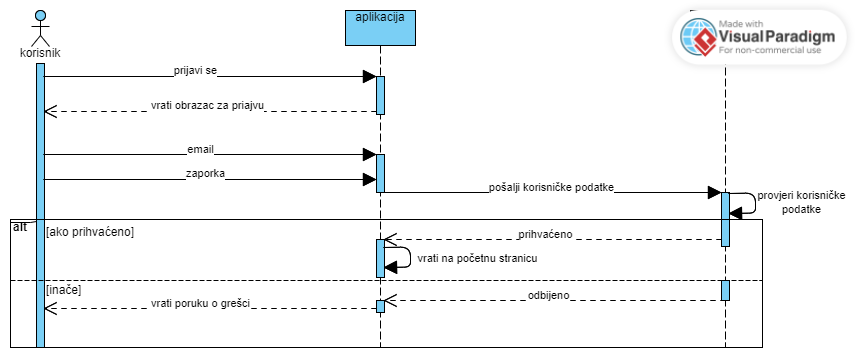
\includegraphics[width=\textwidth]{slike/progiSeqLogin.png} %veličina u odnosu na širinu linije
					\caption{Sekvencijski dijagram - prijava}
					\label{fig:seq1} %label mora biti drugaciji za svaku sliku
				\end{figure}
				
				\begin{figure}[H]
					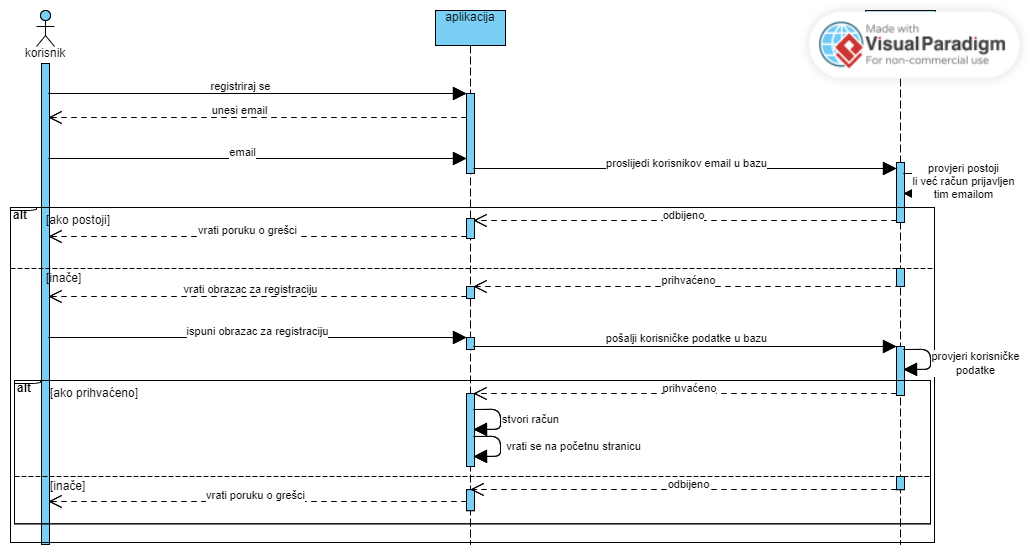
\includegraphics[width=\textwidth]{slike/progiSeqRegister.png} %veličina u odnosu na širinu linije
					\caption{Sekvencijski dijagram - registracija}
					\label{fig:seq2} %label mora biti drugaciji za svaku sliku
				\end{figure}
				\eject
	
		\section{Ostali zahtjevi}
		
			\textbf{\textit{dio 1. revizije}}\\
		 
			 \textit{Nefunkcionalni zahtjevi i zahtjevi domene primjene dopunjuju funkcionalne zahtjeve. Oni opisuju \textbf{kako se sustav treba ponašati} i koja \textbf{ograničenja} treba poštivati (performanse, korisničko iskustvo, pouzdanost, standardi kvalitete, sigurnost...). Primjeri takvih zahtjeva u Vašem projektu mogu biti: podržani jezici korisničkog sučelja, vrijeme odziva, najveći mogući podržani broj korisnika, podržane web/mobilne platforme, razina zaštite (protokoli komunikacije, kriptiranje...)... Svaki takav zahtjev potrebno je navesti u jednoj ili dvije rečenice.}

			 \begin{packed_item}
				\item implementacija jednostavnog i intuitivnog korisničkog sučelja
				\item responzivan dizajn za mogućnost korištenja aplikacije na mobilnim uređajima i računalima
				\item sigurnost podataka u bazi i u komuniciranju s bazom
				\item osiguravanje rada više korisnika u stvarnom vremenu
				\item neispravno korištenje aplikacije ne smije narušiti rad sustava
				\item dizajn treba biti konzistentan kroz sve stranice aplikacije
			\end{packed_item}


			 
			 
			 
	
